%%%%%%%%%%%%%%%%%%%%%%%%%%%%%%%%%%%%%%%%%%%%%%%%%%%%%%%%%%%%%%%%%%%%%%%%%%%%%%%%
\documentclass[
	authors = {{J.~Zhang, L.~Einig}},
	title = {{Introduction to Robotics}},
	department = {{Department of Informatics}},
	group = {{Technical Aspects of Multimodal Systems}},
	type = {{Assignment}},
	id = {{0}},
]{tamsAssignment}

\usepackage{amsmath,amssymb}%math mode extras
\usepackage{graphicx}%pictures and graphics
\usepackage{array}%tables
\usepackage{tabularx}%tables
\usepackage{multicol}%tables
\usepackage{textcomp}%extra icons and symbols
\usepackage{tikz}%drawing
\usepackage{tikz-3dplot}%3d drawing
\tikzset{>=latex}%arrowtip for drawings
\usetikzlibrary{positioning, arrows, patterns, shadows, shapes.geometric, shapes.misc, calc, 3d, decorations.pathmorphing, decorations.markings}%libraries for drawing

\begin{document}
\header{}
%%%%%%%%%%%%%%%%%%%%%%%%%%%%%%%%%%%%%%%%%%%%%%%%%%%%%%%%%%%%%%%%%%%%%%%%%%%%%%%%
%%%%% Edit below %%%%%%%%%%%%%%%%%%%%%%%%%%%%%%%%%%%%%%%%%%%%%%%%%%%%%%%%%%%%%%%
%%%%%%%%%%%%%%%%%%%%%%%%%%%%%%%%%%%%%%%%%%%%%%%%%%%%%%%%%%%%%%%%%%%%%%%%%%%%%%%%
{\centering
	\begin{tabular}{ccc}
		Student Name 1 & Student Name 2 & Student Name 3 \\
		Matriculation No.1 & Matriculation No.2 & Matriculation No.3
	\end{tabular}\\
}

\task{8}{Pyramid}

Your solution here.

\subtask{4}

Your solution here.

\task{}{Some example \LaTeX snippets}

\begin{itemize}
	\item In-Text math mode:
	Rotation by $\psi = 30^\circ$ around $M_{w}$

	\item Matrix in an equation without numbering:\\
	\[
		^AT_B = \begin{bmatrix}
			1/\sqrt{2} & 1/\sqrt{2} & 0 & 1\\
			-1/\sqrt{2} & 1/\sqrt{2} &0 & 1 \\
			0 & 0 & 1 & 0 \\
			0 & 0 & 0 & 1
		\end{bmatrix}
	\]

	\item Matrix in an equation with numbering:\\
	\begin{equation}
		^BT_C = \begin{bmatrix}
			\sqrt{3}/2 & -1/2 & 0 & 2 \\
			1/2 & \sqrt{3}/2 & 0 & 1 \\
			0 & 0 & 1 & 0 \\
			0 & 0 & 0 & 1 \end{bmatrix}
		\end{equation}

	\item Schematics in \LaTeX:\\
	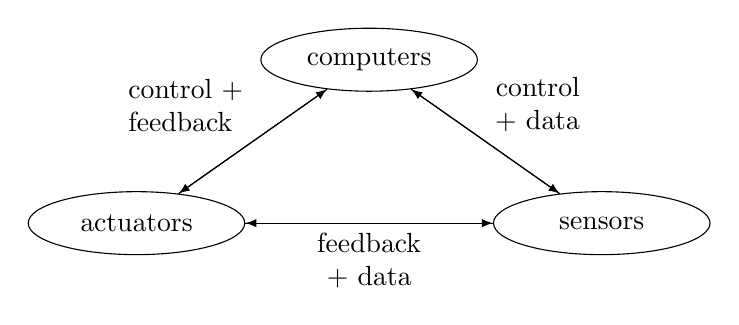
\begin{tikzpicture}
    	\node[draw,ellipse, minimum width=2.75cm, minimum height=.8cm] (computers) {computers};
    	\node[draw,ellipse, minimum width=2.75cm, minimum height=.8cm, below left=1.5cm and 1cm of computers, anchor=north east] (actuators) {actuators};
    	\node[draw,ellipse, minimum width=2.75cm, minimum height=.8cm, below right=1.5cm and 1cm of computers, anchor=north west] (sensors) {sensors};

    	\draw[<->] (computers) -- (actuators);
    	\draw[<->] (computers) -- (sensors);
    	\draw[<->] (sensors) -- (actuators);

    	\draw[] (computers) -- (actuators) node[midway,above left, align=left] {control +\\feedback};
    	\draw[] (computers) -- (sensors) node[midway,above right, align=right] {control\\+ data};
    	\draw[] (sensors) -- (actuators) node[midway,below, align=center] {feedback\\+ data};
	\end{tikzpicture}

	\item Graphics within \LaTeX:\\
	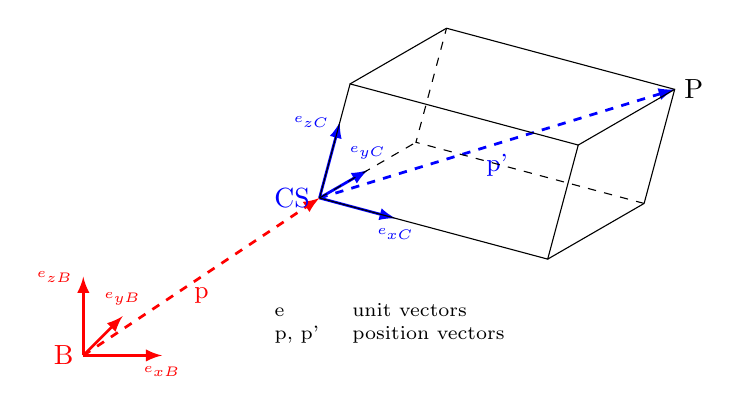
\begin{tikzpicture}
    	\draw[->, red, line width=1pt] (0,0) -- (0,1) node[left] {\tiny{$e_{zB}$}};
    	\draw[->, red, line width=1pt] (0,0) -- (1,0) node[below] {\tiny{$e_{xB}$}};
    	\draw[->, red, line width=1pt] (0,0) -- (.5,.5) node[anchor=south] {\tiny{$e_{yB}$}};;
    	\node[red,anchor=east] at (0,0) {B};
    	\draw[->, red, dashed, line width=1pt] (0,0) -- (3,2) node[midway, below] {\small{p}};

    	\begin{scope}[xshift=3cm,yshift=2cm,rotate=-15]
	        \draw[->, blue, line width=1pt] (0,0) -- (0,1) node[left] {\tiny{$e_{zC}$}};
        	\draw[->, blue, line width=1pt] (0,0) -- (1,0) node[below] {\tiny{$e_{xC}$}};;
        	\draw[->, blue, line width=1pt] (0,0) -- (.5,.5) node[anchor=south] {\tiny{$e_{yC}$}};;
        	\node[blue,anchor=east] at (0,0) {CS};
        	\draw[->, blue, dashed, line width=1pt] (0,0) -- (4,2.5) node[midway, below] {\small{p'}};
        	\node[black,anchor=west] at (4,2.5) {P};


        	\draw[-, black] (0,0) -- (0,1.5) -- (3,1.5) -- (3,0) -- (0,0);
        	\draw[-, black] (1,2.5) -- (4,2.5) -- (4,1) ;
        	\draw[-, black, dashed] (4,1) -- (1,1) -- (1,2.5);
        	\draw[-, black, dashed] (0,0) -- (1,1);
        	\draw[-, black] (0,1.5) -- (1,2.5);
        	\draw[-, black] (3,1.5) -- (4,2.5);
        	\draw[-, black] (3,0) -- (4,1);
    	\end{scope}
    	\node[black,anchor=south west, align=left] at (2,0) {
	        \scriptsize{
            	\begin{tabular}{ll}
	                e & unit vectors \\
                	p, p' & position vectors
            	\end{tabular}
        	}
    	};
	\end{tikzpicture}

	\item 3D-Graphics for experienced \LaTeX users:\\
	\tdplotsetmaincoords{45}{135}
	\begin{tikzpicture}[tdplot_main_coords]
		\draw[->,darkgray] (0,0,0) -- (1,0,0) node[anchor=east]{\tiny x};
		\draw[->,darkgray] (0,0,0) -- (0,1,0) node[anchor=west]{\tiny y};
		\draw[->,darkgray] (0,0,0) -- (0,0,1) node[anchor=south]{\tiny z};

		\tdplotsetrotatedcoords{0}{30}{-30}
		\draw[thick, tdplot_rotated_coords,domain=-2.5:3,smooth,variable=\x,blue,<-] plot (\x,{.5+1.5*cos(\x r)});
		\node[thick, tdplot_rotated_coords,blue] at (-2.7,{.5+1.5*cos(-2.7 r)},0) {\tiny $p_{end}$};
		\node[thick, tdplot_rotated_coords,blue] at (3.2,{.5+1.5*cos(3.2 r)},0) {\tiny $p_{start}$};

		\draw[thick, tdplot_rotated_coords,->] (0,0,0) -- (1,{.5+1.5*cos(1 r)},0) node[near end,below,yshift=-10,xshift=-10] {\tiny $p(t_0)=p_0$};
		\draw[thick, tdplot_rotated_coords,->] (0,0,0) -- (-0.5,{.5+1.5*cos(-0.5 r)},0) node[near end,right,xshift=5,yshift=-10] {\tiny $p(t_0+\Delta t)$};;
		\draw[thick, tdplot_rotated_coords,->] (0,0,0) -- (-1.5,{.5+1.5*cos(-1.5 r)},0) node[near end,above,xshift=-4] {\tiny $p(t_0+\Delta t)$};
	\end{tikzpicture}
\end{itemize}

\end{document}
